\section{Noninteracting controller}

\begin{frame}[shrink=10]{Theory of Noniteracting control}
  Consider a nonlinear control affine system with $m$ inputs and $m$ outputs
  \[
  \vec{\dot{x}} = \vec{f}(\vec{x}) + \sum\limits_{i=1}^{\alert{m}} \vec{g}_{i}(\vec{x}) u_{i}
  \]
  \[
  y_{1} = h_{1}(\vec{x})
  \]
  \[
  \hdots
  \]
  \[
  y_{m} = h_{\alert{m}}(\vec{x})
  \]
  and an initial point $\vec{x}^{0}$
  \par
  The problem of noninteracting control is stated as finding a regular static state feedback
  \[
  \vec{u}(\vec{x})  = \vec{\alpha}(\vec{x}) + \vec{\beta}(\vec{x}) \vec{v} \quad \vec{x} \in B_{\delta}(\vec{x}^0)
  \]
  such that in the resulting closed loop system each output $y_i$ is affected
  only by the corresponding input $v_i$ and not by the others.
\end{frame}

\begin{frame}{Theory of Noniteracting control (continued)}
  Suppose that the system has a vector relative degree $\{r_1, \hdots, r_m\}$ at $\vec{x}^{0}$ hence it admits
  a \emph{normal form} locally around $\vec{x}^{0}$
  \begin{columns}[t]
    \begin{column}{0.5\textwidth}
      \[
      \dot{\xi}_{1}^{i} = \xi_{2}^{i}
      \]
      \[
      \hdots
      \]
      \[
      \dot{\xi}_{r_{i}-1}^{i} = \xi_{r_{i}}^{i}
      \]
      \[
      1 \le i \le m
      \]
      \[
      \begin{bmatrix}
        \dot{\xi}_{r_{1}}^{1}\\
        \vdots\\
        \dot{\xi}_{r_{m}}^{m}\\
      \end{bmatrix}=
      \vec{b}(\vec{\xi},\vec{\eta}) + A(\vec{\xi},\vec{\eta})\vec{u}
      \]
    \end{column}
    \begin{column}{0.5\textwidth}
      \[
      \vec{\dot{\eta}} = \vec{q}(\vec{\xi},\vec{\eta}) + \vec{p}(\vec{\xi},\vec{\eta})\vec{u}
      \]
      \vskip0.3in
      \[
      \begin{bmatrix}
        \vec{\xi}\\
        \vec{\eta}
      \end{bmatrix} = 
      \Phi(\vec{x})
      \]
    \end{column}
  \end{columns}
  \centering
  with $A(\vec{x})$ nonsingular at $\vec{x}^{0}$
\end{frame}

\begin{frame}{Theory of Noniteracting control (continued)}
  \begin{block}{Proposition (Isidori)}
    Suppose
    \[
    L{\vec{g}_j}L_{\vec{f}}^{k}h_{i}(\vec{x}) = 0 \enspace \forall \vec{x} \in B_{\delta}(\vec{x}^0)
    \]
    \[
    1 \le j \le m, \enspace 1 \le i \le m, \enspace k < r_i-1
    \]
    and
    \[
    \begin{bmatrix}
      L_{\vec{g}_1}L_{\vec{f}}^{r_{i-1}}h_i(\vec{x}^{0}) \enspace \hdots \enspace L_{\vec{g}_m}L_{\vec{f}}^{r_i-1}h_i(\vec{x}^{0})
    \end{bmatrix}
    \ne
    \begin{bmatrix}
      0 \enspace \hdots \enspace 0
    \end{bmatrix}
    \enspace 1 \le i \le m
    \]
    Then the noninteracting control problem is solvable iff the matrix $A(\vec{x}^{0})$ is nonsingular,
    i.e. if the system has a vector relative degree $\{r_1, \hdots, r_m\}$ at $\vec{x}^{0}$
  \end{block}
\end{frame}

\begin{frame}{Theory of Noniteracting control (continued)}
  Indeed the regular static feedback
  \[
  \vec{u} = -A^{-1}(\vec{\xi},\vec{\eta})\vec{b}(\vec{\xi},\vec{\eta}) + A^{-1}(\vec{\xi},\vec{\eta})\vec{v}
  \]
  results in the closed loop system
  \begin{columns}[t]
    \begin{column}{0.5\textwidth}
      \[
      \dot{\xi}_{1}^{i} = \xi_{2}^{i}
      \]
      \[
      \hdots
      \]
      \[
      \dot{\xi}_{r_{i}-1}^{i} = \xi_{r_{i}}^{i}
      \]
      \[
      \dot{\xi}_{r_{i}}^{i} = v_{i}
      \]
      \[
      y_{i} = \xi_{1}^{i}
      \]
      \[
      1 \le i \le m
      \]
    \end{column}
    \begin{column}{0.5\textwidth}
      \[
      \vec{\dot{\eta}}  = \hat{\vec{q}}(\vec{\xi},\vec{\eta}) + \hat{\vec{p}}(\vec{\xi},\vec{\eta})\vec{v}
      \]
    \end{column}
  \end{columns}
\end{frame}

\begin{frame}{Application of the Noniteracting control}
  For the system under examination
  \[
  \begin{cases}
    \begin{split}
      \dot{\vec{x}} &= \vec{f}(\vec{x}) + g(\vec{x})\vec{u}\\
      &=\vec{f}(\vec{x}) +
      \begin{bmatrix}
        0_{3\times3} \\
        \left(B(\theta_2,\theta_3) ^ {-1}\right)_{(:, 4:6)}
      \end{bmatrix}\vec{u}\\
    \end{split}\\
    \vec{y} = \vec{h}(\vec{x}) =
    \begin{bmatrix}
      \theta_1 &
      \theta_2 &
      \theta_3
    \end{bmatrix} \transpose
  \end{cases}
  \]
  it can be found that
  \[
  L_{\vec{g}_{j}}L_{\vec{f}}^{0}h_{i} =
  L_{\vec{g}_{j}}h_{i} = 
  \begin{bmatrix}
    \vec{e}_i & 0_{6x1}
  \end{bmatrix}
  \vec{g}_j
  =
  g_{j}^{i} = 0
  \qquad 1 \le j \le 3, \enspace 1 \le i \le 3
  \]

\end{frame}

\begin{frame}{Existence of a vector relative degree}
  Also 
  \[
  \frac{\mathrm{d}^{2}}{\mathrm{d}t^{2}}\vec{y} = 
  \begin{bmatrix}
    \ddot{\theta_1}\\
    \ddot{\theta_2}\\
    \ddot{\theta_3}
  \end{bmatrix} =
  \vec{b}(\vec{x}) + A(\vec{x}) \vec{u}
  \]
  where
  \[
  \vec{b}(\vec{x}) = \vec{f}(\vec{x})_{(4:6)}
  \]
  and
  \[
  A(\vec{x}) = \left(B(\theta_2,\theta_3) ^ {-1}\right)_{(1:3, 4:6)}
  \]
\end{frame}

\begin{frame}{Existence of a vector relative degree (continued)}
  \centering
  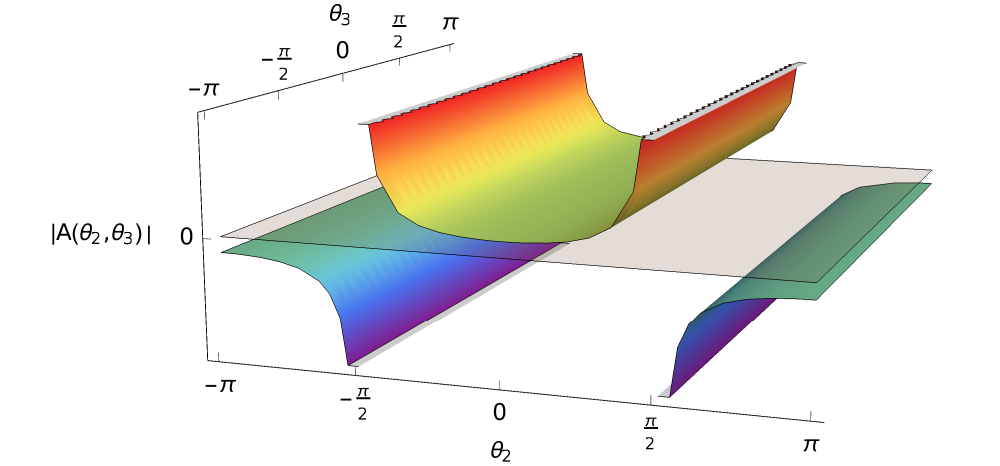
\includegraphics[scale=0.4]{detA.png}
  \[
  |A| \ne 0 \enspace \forall \theta_2, \theta_3 \implies \{r_1, r_2, r_3\} = \{2,2,2\} \enspace \forall \vec{x}
  \]
  The resulting standard noninteractive feedback is
  \[
  \vec{u}_{NIC} = -\left(B(\theta_2,\theta_3) ^ {-1}\right)_{(1:3, 4:6)}^{-1}
  (\vec{f}_{(4:6)}(\vec{x}) - \vec{v} )
  \]
\end{frame}

\begin{frame}[shrink=10]{Unobservable part of the system}
  The unobservable part of the system can be obtained by completely specifying
  the coordinate transformation $\Phi$
  \[
  \vec{y} =
  \begin{bmatrix}
    \theta_1 &
    \theta_2 &
    \theta_3
  \end{bmatrix}\transpose
  \implies
  \Phi(\vec{x})_{1:6} =
  \begin{bmatrix}
    \theta_1 & \dot{\theta}_1 &  \theta_2 & \dot{\theta}_2 &
    \theta_3 & \dot{\theta}_3
  \end{bmatrix}\tranpose
  \]
  The remaining part is chosen as
  \[
  \Phi(\vec{x})_{1:6} =
  \begin{bmatrix}
    \dot{q}_x & \dot{q}_y & \dot{q}_z
  \end{bmatrix}\transpose
  \]
  i.e. the unobservable part of the closed loop system is the closed loop dynamics of the
  flywheels
  \[
  \begin{split}
    \dot{\vec{\eta}} &=
    \begin{bmatrix}
      \ddot{q}_{x}\\
      \ddot{q}_{y}\\
      \ddot{q}_{z}
    \end{bmatrix}
    = \vec{f}_{(7:9)}(\vec{x}) + \left(B(\theta_2,\theta_3) ^ {-1}\right)_{(4:6, 4:6)} \vec{u}_{NIC}\\
    &=\vec{f}_{(7:9)}(\vec{x}) - \left(B(\theta_2,\theta_3) ^ {-1}\right)_{(4:6, 4:6)}
    \left(B(\theta_2,\theta_3) ^ {-1}\right)_{(1:3, 4:6)}^{-1}
    (\vec{f}_{(4:6)}(\vec{x}) - \vec{v})\\
    &=\hat{\vec{q}}(\vec{x}) + \hat{\vec{p}}(\theta_{2},\theta_{3})\vec{v}
  \end{split}
  \]
\end{frame}

\begin{frame}{Yaw motion while balancing on a corner}
  Consider a rotation about the $z$ axis of the inertial
  reference frame $\{S\}$ while the balance on one of the corner is maintained
  \begin{center}
    \includemedia[
      activate=pageopen,
      width=90pt,height=90pt,
      addresource=videos/cubli_yaw_noerr.mp4,
      flashvars={%
        src=videos/cubli_yaw_noerr.mp4
        &scaleMode=stretch&autoPlay=true&loop=true
        &hideBar=true}
    ]{}{StrobeMediaPlayback.swf}
  \end{center}
\end{frame}

\begin{frame}{Yaw motion while balancing on a corner (continued)}
  A suitable control law $\vec{v}$ is
  {\small
    \[
    \begin{split}
      &v_1(t) = \ddot{\theta}_1^{des}(t) + k_d(\dot{\theta}_1^{des}(t) - \dot{\theta}_1(t)) + k_p (\theta_1^{des}(t) - \theta_1(t))\\
      &v_2(t) = - k_d\dot{\theta}_2(t) + k_p \left(-\mathrm{atan}\frac{\sqrt{2}}{2} - \theta_2(t)\right)\\
      &v_3(t) = - k_d\dot{\theta}_3(t) + k_p \left(\frac{\pi}{4} - \theta_3(t)\right)
    \end{split}
    \]
  }
  where
  \[
  \theta_1^{des}(t) = a_0 + a_1 t + a_2 t^2 + a_3 t^3 + a_4 t^4 + a_5 t^5
  \]
  with boundary conditions
  \[
  \begin{split}
    &\theta_1^{des}(0) \in [-\pi, \pi) \quad \dot{\theta}_1^{des}(0)= 0 \quad \ddot{\theta}_1^{des}(0) = 0\\
      &\theta_1^{des}(t_{f}) \in [-\pi, \pi)  \quad \dot{\theta}_1^{des}(t_{f})= 0 \quad \ddot{\theta}_1^{des}(t_{f}) = 0
  \end{split}
  \]
\end{frame}

\begin{frame}{Results}
  \[\theta_1^{des}(0) = \SI{0}{\degree} \rightarrow \theta_1^{des}(2) = \SI{100}{\degree}
  \rightarrow \theta_1^{des}(4) = \SI{0}{\degree}\]
  \[k_p = 10 \enspace k_d = 0.1\]
  \begin{center}
    \includemedia[
      activate=pageopen,
      width=288pt,height=162pt,
      addresource=videos/cubli_yaw.mp4,
      flashvars={%
        src=videos/cubli_yaw.mp4
        &scaleMode=stretch&autoPlay=true}
    ]{}{StrobeMediaPlayback.swf}
  \end{center}
\end{frame}

\begin{frame}{Results (continued)}
  The flywheel velocities $\vec{\eta}(t)$ which are
  solution to the differential equation
  \[
  \begin{cases}
    \dot{\vec{\eta}} = \hat{\vec{q}}(\vec{x}) + \hat{\vec{p}}\left(-\mathrm{atan}\frac{\sqrt{2}}{2},\frac{\pi}{4}\right)\vec{v}_{PD}\\
    \vec{\eta}(0) = \vec{0}
  \end{cases}
  \]
  are bounded and tends to zero
  \par
  \centering
  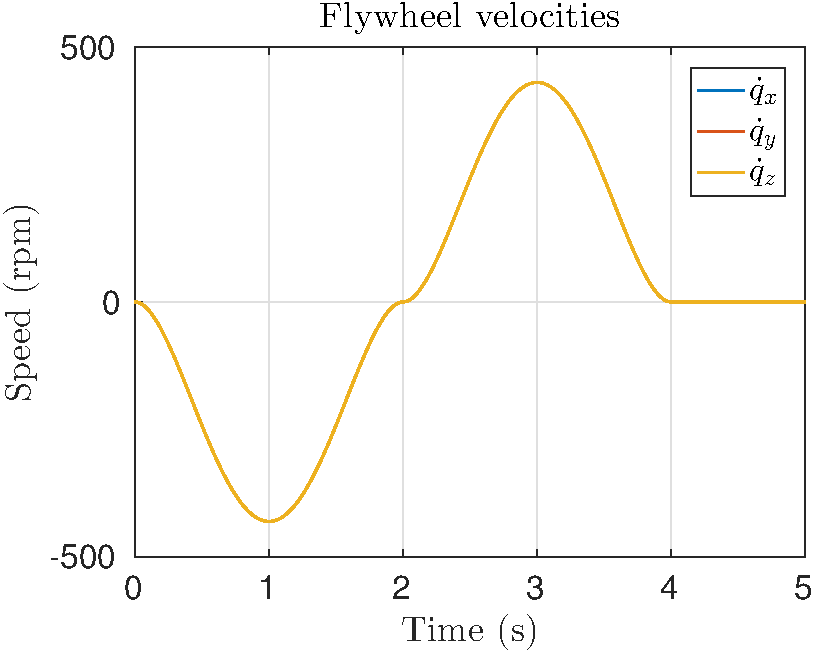
\includegraphics[scale=0.4]{fly_wheel2}
\end{frame}

\begin{frame}{Use of an alternative Euler parametrization}
\end{frame}

\begin{frame}{Results}
  \vskip0.1in
  \begin{columns}
    \begin{column}{0.45\textwidth}
      \begin{itemize}
      \item[-]$k_p = 2500$, $k_d = 50$
      \item[-]rotation of $\SI{180}{\degree}$ in $\SI{4}{\second}$
      \item[-]LQR control actived at $t = \SI{5}{\second}$ 
      \end{itemize}
    \end{column}
    \begin{column}{0.45\textwidth}
      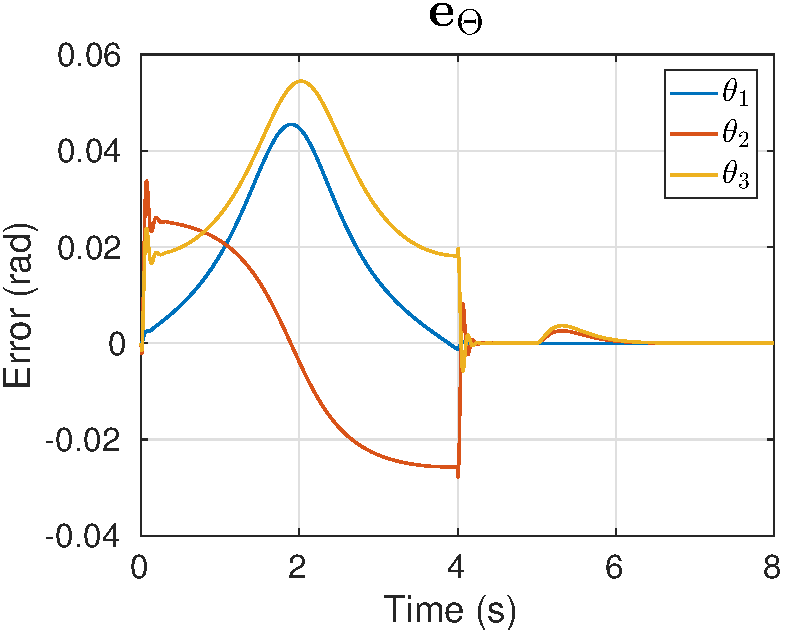
\includegraphics[width=\columnwidth]{error_lqr}
    \end{column}
  \end{columns}
  \begin{columns}
    \begin{column}{0.45\textwidth}
      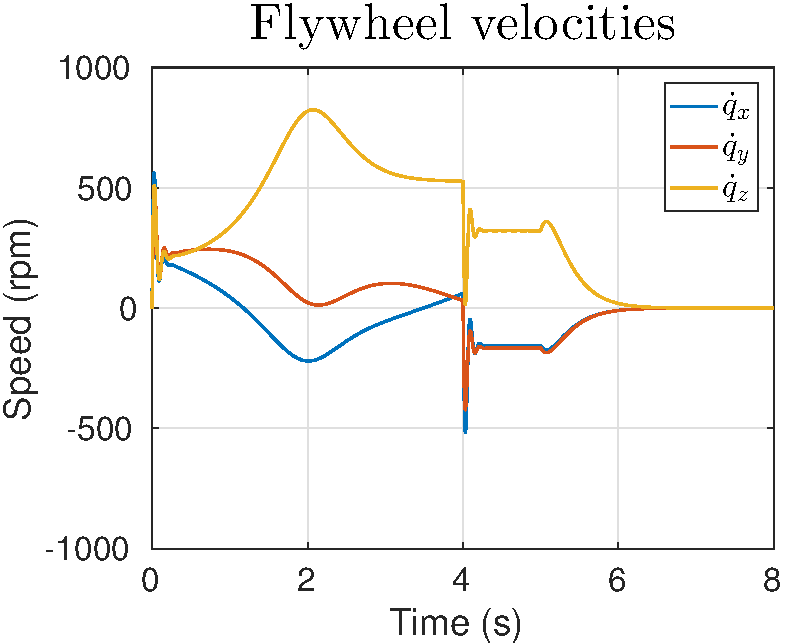
\includegraphics[width=\columnwidth]{fly_wheel_lqr}
    \end{column}
    \begin{column}{0.45\textwidth}
      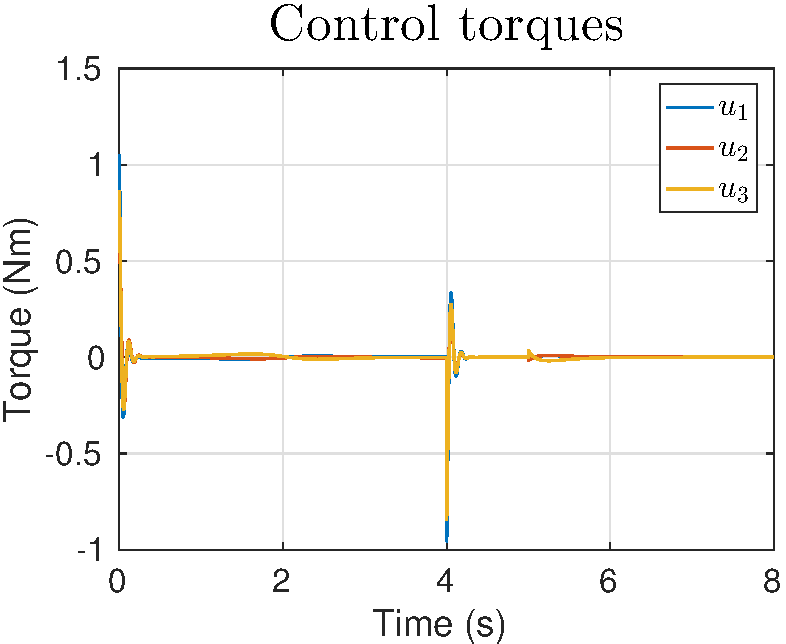
\includegraphics[width=\columnwidth]{input_lqr}
    \end{column}
  \end{columns}
\end{frame}

%% \begin{frame}{Results ($k_p = 2500$, $k_d = 50$)}
%%   \centering
%%   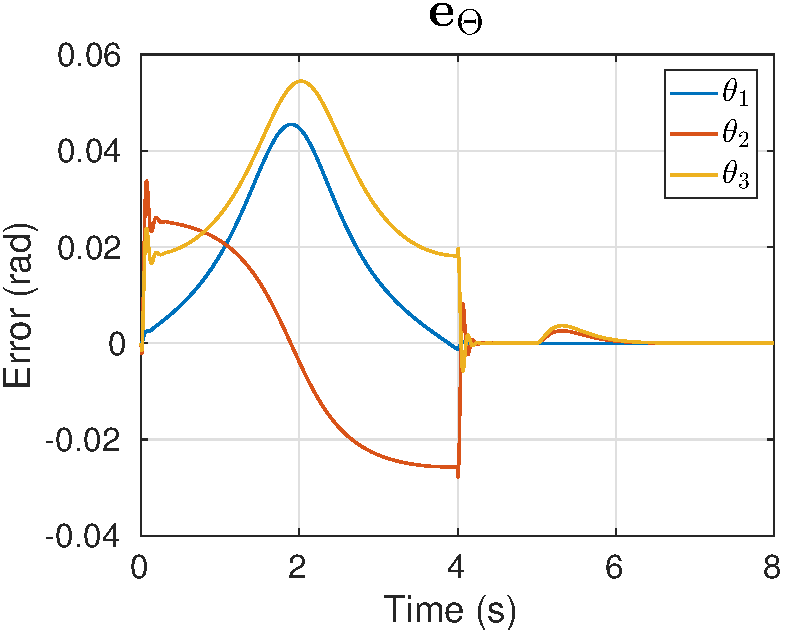
\includegraphics[scale=0.4]{error_lqr}
%%   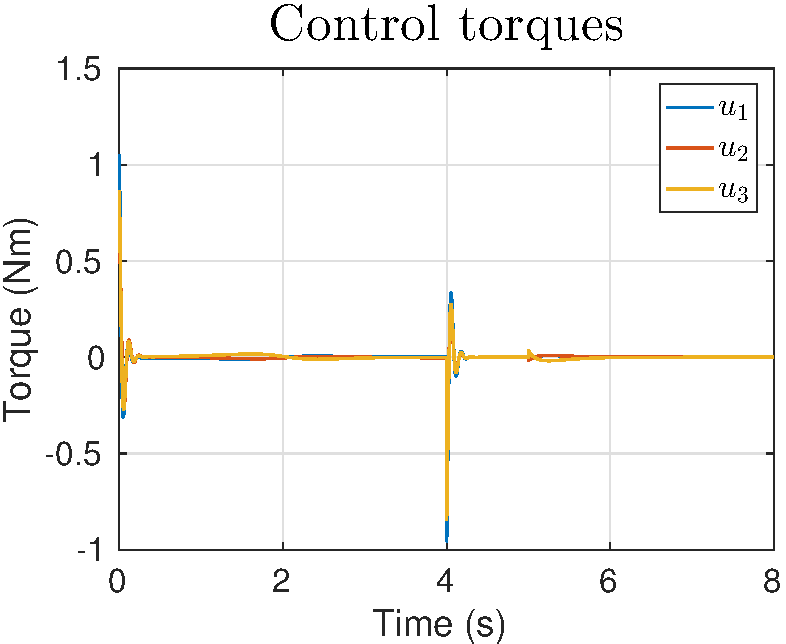
\includegraphics[scale=0.4]{input_lqr}
%% \end{frame}

%% \begin{frame}{Results}
%%   The LQR control is actived at $t = \SI{5}{\second}$
%%   \par
%%   \centering
%%   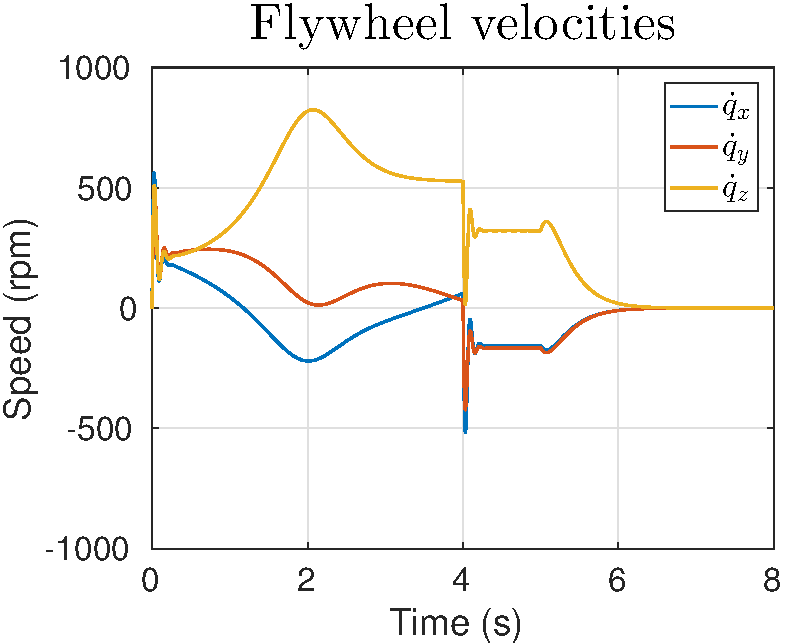
\includegraphics[scale=0.6]{fly_wheel_lqr}
%% \end{frame}

\begin{frame}{Results}
  The outcome of the switch to the LQR controller
  is shown for several angles of rotation and several durations of the movement
  \par
  \centering
  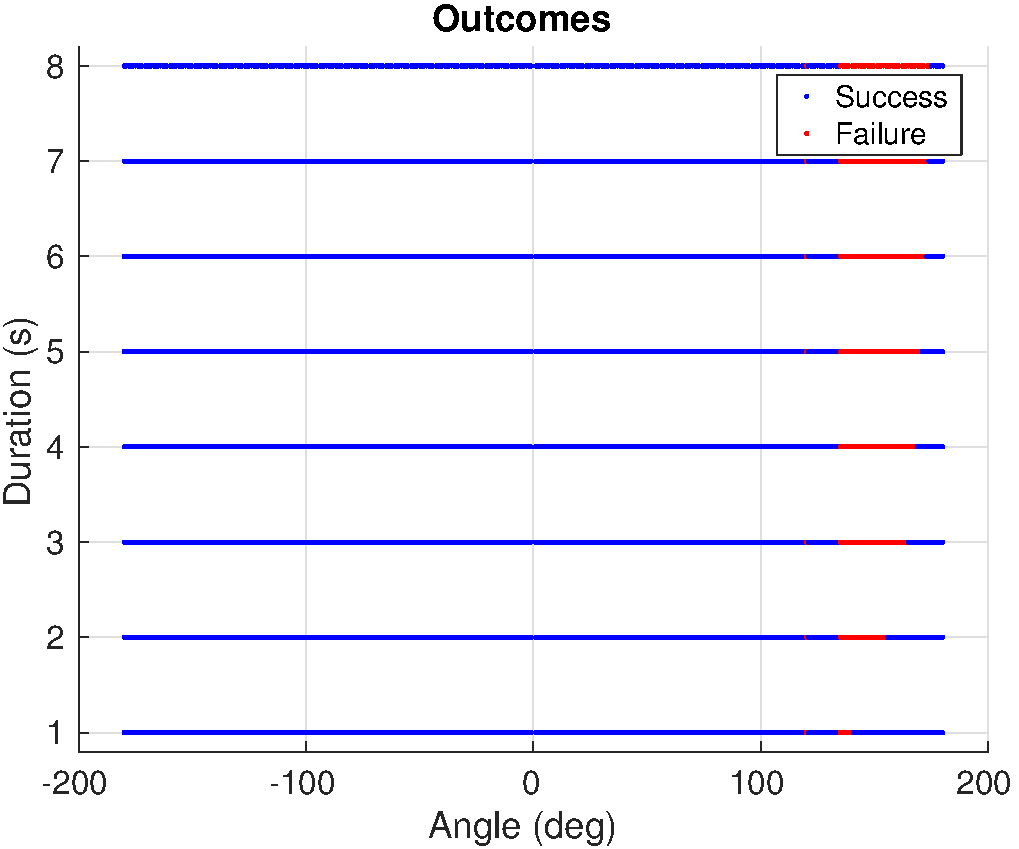
\includegraphics[scale=0.46]{simulation_lqr}
\end{frame}

\begin{frame}{Results}
  The failures happen when the flywheel velocities are too high as expected
  \par
  \centering
  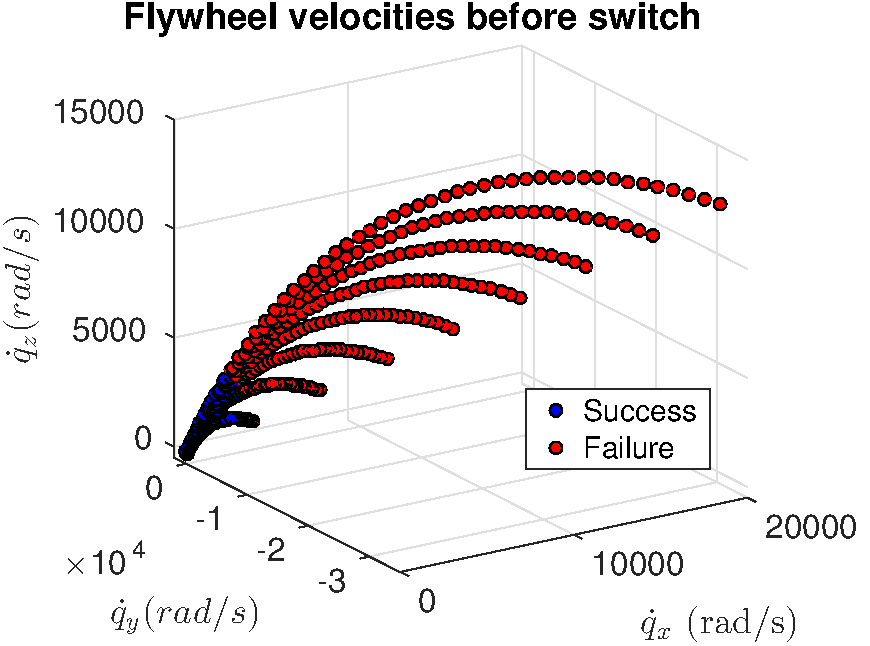
\includegraphics[scale=0.62]{simulation_lqr_velocities}
\end{frame}

